\documentclass{homework}
\newcommand{\R}{\textbf{R}}
\newcommand{\dee}{\;\text{d}}
\usepackage{enumitem}

\newcommand{\hwclass}{Math 6418}
\newcommand{\hwname}{Jacob Hauck}
\newcommand{\hwtype}{Homework}

\newcommand{\dist}{\mathcal{D}}

\newcommand{\hwnum}{1}
\renewcommand{\questiontype}{Problem}

\begin{document}
	\maketitle
	
	\question 
	
	Consider the IVP
	\begin{equation}
		y' = 3 + e^{-t} - y, \quad t > 0; \qquad y(0) = 1.
	\end{equation}
	The code to answer the following questions is found in \lstinline{problem1_calculations.m}. The output from running this script is copied into \lstinline{problem1_output.txt}.
	
	\begin{arabicparts}
		\questionpart Multiplying both sides by the integrating factor $e^t$ gives
		\begin{equation}
			y'e^t + ye^t = 3e^t + 1.
		\end{equation}
		The left-hand side is $(ye^t)'$, so integrating on both sides gives
		\begin{equation}
			ye^t = 3e^t + t + C,
		\end{equation}
		for some constant $C$, so $y(t) = 3 + (t + C)e^{-t}$. The initial condition $y(0) = 1$ implies that $C = -2$, so
		\begin{equation}
			y(t) = 3 + (t-2)e^{-t}.
		\end{equation}
		
		\questionpart
		\begin{enumerate}[label=({\bf\alph*})]
			\item To discretize the IVP on $[0,2]$ using the forward Euler method, we need to have an evenly-spaced set of time samples $\{t_i\}_{i=0}^n$ defined by
			\begin{equation}
				t_i = \begin{cases}
					0 & i = 0 \\
					t_{i-1} + k, & i \ge 1,
				\end{cases}, \qquad i = 0,1,\dots,n.
			\end{equation}
			The value $k$ is the step size and is chosen so that $t_n = 2$; that is, $k = \frac{2}{n}$. We will attempt to find an approximation $\{y_i\}_{i=0}^n$ of the values $\{y(t_i)\}_{i=0}^n$. To find $\{y_i\}$, we create and solve a system of equations from the ODE by approximating $y'(t_i)$ by the forward difference $y'(t_i) \approx \frac{y(t_{i+1}) - y(t_i)}{k}$, where $i < n$. Since we know that $y(0) = 1$ from the initial condition, we are led to the scheme
			\begin{equation}
				\begin{cases}
					y_0 = 1 &\\
					\frac{y_{i+1} - y_i}{k} = 3 + e^{-t_i} - y_i, & 0\le i < n,
				\end{cases}
			\end{equation}
			which allows to write an explicit recursive formula for $y_i$:
			\begin{equation}
				\begin{cases}
					y_0 = 1 &\\
					y_{i+1} = y_i + k(3 + e^{-t_i} - y_i), & 0\le i < n.
				\end{cases}
			\end{equation}
			The code for this scheme can be found in \lstinline{problem1_fe.m}.
			
			\item According the output from \lstinline{problem1_output.txt}, the numerical value of $y(2)$ is 3.012754.
			\item Below (Figure \ref{fig:p12c}) is the plot generated by \lstinline{problem1_calculations.m}.
			\begin{figure}[h]
				\centering
				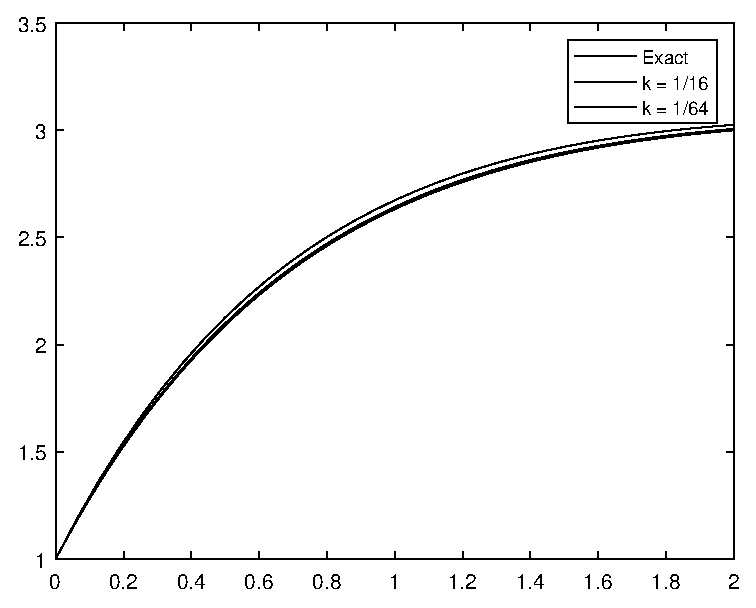
\includegraphics{p1.2c.eps}
				\caption{The exact solution of the ODE and the numerical approximations using the forward Euler method with $k = \frac{1}{16}$ and $k = \frac{1}{64}$.}
				\label{fig:p12c}
			\end{figure}
		\end{enumerate}
		
		\questionpart
		\begin{enumerate}[label=({\bf\alph*})]
			\item To discretize the IVP on $[0,2]$ using the backward Euler method, we need to have an evenly-spaced set of time samples $\{t_i\}_{i=0}^n$ defined by
			\begin{equation}
				t_i = \begin{cases}
					0 & i = 0 \\
					t_{i-1} + k, & i \ge 1,
				\end{cases}, \qquad i = 0,1,\dots,n.
			\end{equation}
			The value $k$ is the step size and is chosen so that $t_n = 2$; that is, $k = \frac{2}{n}$. We will attempt to find an approximation $\{y_i\}_{i=0}^n$ of the values $\{y(t_i)\}_{i=0}^n$. To find $\{y_i\}$, we create and solve a system of equations from the ODE by approximating $y'(t_i)$ by the backward difference $y'(t_i) \approx \frac{y(t_i) - y(t_{i-1})}{k}$, where $i > 0$. Since we know that $y(0) = 1$ from the initial condition, we are led to the scheme
			\begin{equation}
				\begin{cases}
					y_0 = 1 &\\
					\frac{y_i - y_{i-1}}{k} = 3 + e^{-t_i} - y_i, & 0 < i \le n,
				\end{cases}
			\end{equation}
			which allows to write an explicit recursive formula for $y_i$:
			\begin{equation}
				\begin{cases}
					y_0 = 1 &\\
					y_i = \frac{y_{i-1} + k(3 + e^{-t_i})}{1+k}, & 0 < i \le n.
				\end{cases}
			\end{equation}
			The code for this scheme can be found in \lstinline{problem1_be.m}.
			
			\item According the output from \lstinline{problem1_output.txt}, the numerical value of $y(2)$ is 2.987379.
			\item Below (Figure \ref{fig:p13c}) is the plot generated by \lstinline{problem1_calculations.m}.
			\begin{figure}[h]
				\centering
				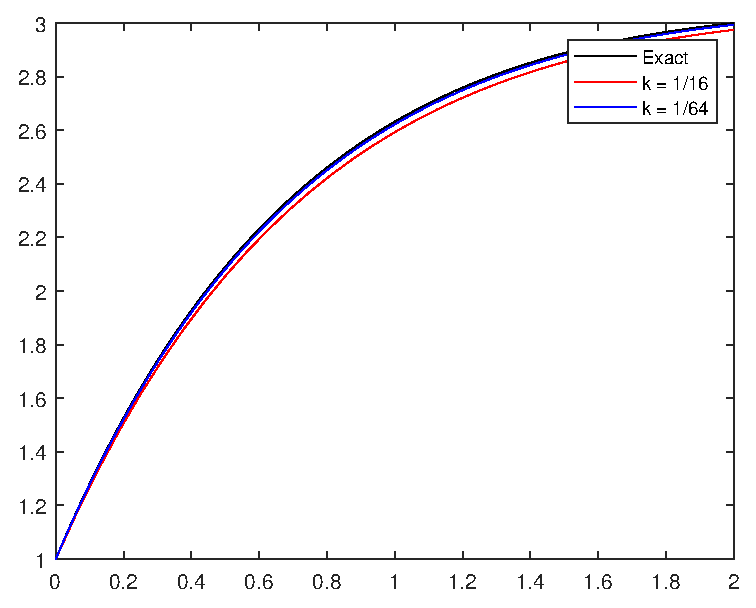
\includegraphics{p1.3c.eps}
				\caption{The exact solution of the ODE and the numerical approximations using the forward Euler method with $k = \frac{1}{16}$ and $k = \frac{1}{64}$.}
				\label{fig:p13c}
			\end{figure}
		\end{enumerate}
		
		\questionpart Below (Table \ref{table:p1}) are numerical errors at $t=1$ for the forward and backward Euler methods at different step sizes.
		
		\begin{table}[htb]
			\centering
			\begin{tabular}{@{}lll@{}}
				\toprule
				Time step ($k$) & Forward Euler error & Backward Euler error \\
				\midrule
				1/4 & 0.105516 & 0.097216 \\
				1/8 & 0.051788 & 0.049683 \\
				1/16 & 0.025638 & 0.025109 \\
				1/32 & 0.012754 & 0.012621 \\
				1/64 & 0.006360 & 0.006327 \\
				1/128 & 0.003176 & 0.003168 \\
				1/256 & 0.001587 & 0.001585 \\
				1/512 & 0.000793 & 0.000793 \\
				\bottomrule
			\end{tabular}
			\caption{Numerical errors in $t=2$; comparison of forward and backward Euler methods}
			\label{table:p1}
		\end{table}
	\end{arabicparts}
	
	\question
	
	Consider the IVP
	\begin{equation}
		y' = \frac{3t^2+10t+1}{2(y+1)}, \quad t > 0; \qquad y(0) = -2.
	\end{equation}
	The code to answer the parts of this question can be found in \lstinline{problem2_calculations.m}, and the output from running this script has been copied to \lstinline{problem2_output.txt}.
	
	\begin{arabicparts}
		\questionpart Multiplying both sides by $2(y+1)$ gives
		\begin{equation}
			2(y+1)(y+1)' = 3t^2+10t+1.
		\end{equation}
		The left-hand side is $\left((y+1)^2\right)'$, so integrating on both sides gives
		\begin{equation}
			(y+1)^2 = t^3+5t^2+t+C
		\end{equation}
		for some constant $C$. The initial condition $y(0) = -2$ implies that $C = 1$. Therefore,
		\begin{equation}
			y(t) = -1 \pm \sqrt{t^3+5t^2+t+1}.
		\end{equation}
		The initial condition forces us to choose a negative sign after taking the square root; thus,
		\begin{equation}
			y(t) = -1 - \sqrt{t^3+5t^2+t+1}.
		\end{equation}
		
		\questionpart To discretize the IVP on $[0,1]$ using the backward Euler method, we need to have an evenly-spaced set of time samples $\{t_i\}_{i=0}^n$ defined by
		\begin{equation}
			t_i = \begin{cases}
				0 & i = 0 \\
				t_{i-1} + k, & i \ge 1,
			\end{cases}, \qquad i = 0,1,\dots,n.
		\end{equation}
		The value $k$ is the step size and is chosen so that $t_n = 1$; that is, $k = \frac{1}{n}$. We will attempt to find an approximation $\{y_i\}_{i=0}^n$ of the values $\{y(t_i)\}_{i=0}^n$. To find $\{y_i\}$, we create and solve a system of equations from the ODE by approximating $y'(t_i)$ by the backward difference $y'(t_i) \approx \frac{y(t_i) - y(t_{i-1})}{k}$, where $i > 0$. Since we know that $y(0) = 1$ from the initial condition, we are led to the scheme
		\begin{equation}
			\begin{cases}
				y_0 = 1 &\\
				\frac{y_i - y_{i-1}}{k} = \frac{3t_i^2+10t_i + 1}{2(y_i + 1)}, & 0 < i \le n,
			\end{cases}
		\end{equation}
		which allows to write an implicit recursive formula for $y_i$:
		\begin{equation}
			\begin{cases}
				y_0 = 1 &\\
				2(y_i+1)(y_i-y_{i-1}) - k(3t_i^2+10t_i+1) = 0, & 0 < i \le n.
			\end{cases}
		\end{equation}
		We can solve the implicit equation for $y_i$ numerically using Newton's method. Indeed, if we set
		\begin{equation}
			f_i(y) = 2(y+1)(y-y_{i-1}) - k(3t_i^2+10t_i+1), \qquad 0 < i\le n,
		\end{equation}
		then finding $y_i$ is equivalent to finding the root of $f_i$. Newton's method is easy to apply once we note that $f_i'(y) = 2(y-y_{i-1}) + 2(y+1)$.
		
		The code for this scheme can be found in \lstinline{problem2_be.m}, and it refers to the \lstinline{newton.m} script to run Newton's method.
		
		\questionpart When $k=\frac{1}{16}$ and the numerical tolerance for Newton's method is $\varepsilon = 0.1$, the numerical value of $y(1)$ is $-3.812471$, according to \lstinline{problem2_output.txt}.
		
		\questionpart When $k=\frac{1}{16}$ and the numerical tolerance for Newton's method is $\varepsilon = 10^{-8}$, the numerical value of $y(1)$ is $-3.772976$, according to \lstinline{problem2_output.txt}.
		
		\questionpart Below (Table \ref{table:p2}) are the numerical errors at $t=2$ for different step sizes and Newton's method tolerances.
		\begin{table}[htb]
			\centering
			\begin{tabular}{@{}llll@{}}
				\toprule
				Time step ($k$) & $\varepsilon = 0.1$ error & $\varepsilon=10^{-3}$ error & $\varepsilon =10^{-8}$ error \\
				\midrule
				1/4 & 0.414940 & 0.417989 & 0.417989 \\
				1/8 & 0.211888 & 0.215835 & 0.215836 \\
				1/16 & 0.101119 & 0.109862 & 0.109862 \\
				1/32 & 0.015956 & 0.055450 & 0.055451 \\
				1/64 & 0.007944 & 0.027855 & 0.027860 \\
				1/128 & 0.003964 & 0.013964 & 0.013964 \\
				1/256 & 0.001980 & 0.006991 & 0.006991\\
				1/512 & 0.000989 & 0.003497 & 0.003498 \\
				\bottomrule
			\end{tabular}
			\caption{Numerical errors at $t=1$}
			\label{table:p2}
		\end{table}
	\end{arabicparts}
\end{document}